%%%%%%%%%%%%%%%%%%%%%%%%%%%%%%%%%%%%%%%%%
% Short Sectioned Assignment
% LaTeX Template
% Version 1.0 (5/5/12)
%
% This template has been downloaded from:
% http://www.LaTeXTemplates.com
%
% Original author:
% Frits Wenneker (http://www.howtotex.com)
%
% License:
% CC BY-NC-SA 3.0 (http://creativecommons.org/licenses/by-nc-sa/3.0/)
%
%%%%%%%%%%%%%%%%%%%%%%%%%%%%%%%%%%%%%%%%%

%------------------------------------------------------------------------------
%	PACKAGES AND OTHER DOCUMENT CONFIGURATIONS
%------------------------------------------------------------------------------

\documentclass[paper=a4, fontsize=11pt]{scrartcl} % A4 paper and 11pt font size

\usepackage[T1]{fontenc} % Use 8-bit encoding that has 256 glyphs
%\usepackage{fourier} % Use the Adobe Utopia font for the document - comment this line to return to the LaTeX default
\usepackage[english]{babel} % English language/hyphenation
\usepackage{amsmath,amsfonts,amsthm} % Math packages

\usepackage[font=small,labelfont=bf,margin=1cm]{caption}
\usepackage{verbatim}
\usepackage[utf8]{inputenc} % Needed to support swedish "åäö" chars
\usepackage{titling} % Used to re-style maketitle
\usepackage{enumerate}
\usepackage{lipsum} % Used for inserting dummy 'Lorem ipsum' text into the template

\usepackage{tabularx}
\usepackage{hyperref}
\usepackage{url}
\usepackage{graphicx}
\usepackage[left=2.5cm, right=2.5cm]{geometry} % margins for title page. changed below.

\usepackage{sectsty} % Allows customizing section commands
\allsectionsfont{\normalfont} % Make all sections centered, the default font and small caps

\usepackage{fancyhdr} % Custom headers and footers
\pagestyle{fancyplain} % Makes all pages in the document conform to the custom headers and footers
\fancyhead{} % No page header - if you want one, create it in the same way as the footers below
\fancyfoot[L]{} % Empty left footer
\fancyfoot[C]{} % Empty center footer
\fancyfoot[R]{\thepage} % Page numbering for right footer
\renewcommand{\headrulewidth}{0pt} % Remove header underlines
\renewcommand{\footrulewidth}{0pt} % Remove footer underlines
\setlength{\headheight}{13.6pt} % Customize the height of the header

\numberwithin{equation}{section} % Number equations within sections (i.e. 1.1, 1.2, 2.1, 2.2 instead of 1, 2, 3, 4)
\numberwithin{figure}{section} % Number figures within sections (i.e. 1.1, 1.2, 2.1, 2.2 instead of 1, 2, 3, 4)
\numberwithin{table}{section} % Number tables within sections (i.e. 1.1, 1.2, 2.1, 2.2 instead of 1, 2, 3, 4)

\setlength\parindent{0pt} % Removes all indentation from paragraphs - comment this line for an assignment with lots of text

\usepackage{fancyvrb}
\DefineShortVerb{\|}


\posttitle{\par\end{center}} % Remove space between author and title
%----------------------------------------------------------------------------------------
% TITLE SECTION
%----------------------------------------------------------------------------------------

\title{ 
\huge Laboration 3 \\ Minneshantering v. 4 \\ % The assignment title
\vspace{10pt}
\normalfont \normalsize 
\textsc{ID2200 - Operating Systems } \\ [25pt] %
}

\author{Gustaf Lindstedt \\ glindste@kth.se \\ 910301-2135 \and Martin Runelöv \\ mrunelov@kth.se \\ 900330-5738}

\date{\vspace{8pt}\normalsize\today} % Today's date or a custom date

\begin{document}

\maketitle

%------------------------------------------------------------------------------
\section{Inledning}

% OBS! Se till så att filerna är läsbara för assistenterna (se 3.4 ).
Koden finns tillgänglig i följande sökväg: |/afs/ict.kth.se/home/m/r/mrunelov/os/lab3/|,

samt i appendix. Körinstruktioner finns i filen README.txt


% Verksamhetsberättelse och synpunkter på laborationen. Beskriv arbetets utveckling. Hade du problem med verktygen,
% kompilatorn m.fl.? Hur lång tid har arbetet tagit? Skriv dina förslag till förändringar, idéer etc. Tyck fritt! 
% Vi är angelägna om att få respons, så att vi kan förbättra till nästa år.

% Uppskattning av tidsåtgång och eventuella kommentarer kring laborationen
\subsection{Verksamhetsberättelse}

Vi började genom att studera implementationen i The C Programming language.
Den användes som mall och rättesnöre när vi implementerade vår egna.
Efter att malloc och free implementerats implementerade vi realloc som utnyttjade dom.
När dessa delar klarade sina tester implementerade vi både Best-fit och Worst-fit
algoritmerna för malloc.
Den sista stora additionen till vår implementation var att vi började hålla reda på
även allokerade areor och inte bara lediga utrymmen.
Detta för att kunna identifiera felaktiga anrop till free. \\

Resten av tiden har spenderats på att förfina tester och skript för att kunna sammanställa
grafer och att utvärdera algoritmerna.\\

Tidsåtgång\dots \\


\subsection{Synpunkter}
gprof fungerar inte längre på Mac OS X, och skolans datorer ger en inte tillräckligt med minne för att göra utförliga tester med gprof.
Dessutom skulle vi uppskatta om det fanns ett tydligt exempel på gprof-användning då detta har en tendens att vara krångligt.\\

Det är lite förvirrande att systemets malloc har någon optimering som gör att minnesåtgången blir 0 i alla tester. 
Detta kanske inte gäller alla system, men det borde kanske nämnas i labbpeket för att göra folk beredda på det.\\

Testfilerna är väldigt otydliga med huruvida man har klarat ett test eller inte. Om man kollar i källkoden kan man
oftast räkna ut vad som menas, men det borde inte behövas.
Precis som MERGE-testet borde samtliga tester avslutas med antingen |Test passed OK| eller |Test failed|.
En sådan text per deltest vore ännu bättre. 

Det är också förvirrande med texten |worst case calculation| i MEMORY-testet. Det verkar som att $> 2.0*\text{worst-case}$ 
anses vara ett misslyckande, men man får lätt intrycket att man ska ligga $< 1.0$.


\section{Förberedelsefrågor}

\begin{enumerate}[1)]
\item{mmap:}

Adress-parametern till |mmap| specificerar en virtuell adress som är ett förslag till var |mmap| ska skapa en ny mappning.
|mmap| kommer att skapa en mappning på en närliggande sida.

Om adressen är |NULL| väljer kerneln adress.\\

|mmap| returnerar en pekare till det mappade området, eller |MAP_FAILED| om mappningen misslyckades.\\

Man måste specificera någon av flaggorna |MAP_SHARED| eller |MAP_PRIVATE|. |MAP_SHARED| innebär att
uppdateringar av mappningen är synlig för andra processer som har samma mappning. |MAP_PRIVATE| skapar en privat copy-on-write-mappning.
\end{enumerate}

%------------------------------------------------------------------------------
\section{Problembeskrivning}


%------------------------------------------------------------------------------
\section{Programbeskrivning}

% Har nästan förstått det här. Men är lite osäker på vad dom vill.
% Det nedan + motsvarande förberedelsefrågor-del kan ses som anteckningar tills vidare...
%
% Det är lite oklart hur det hela ska funka.
% sbrk ger oss program break, men __endHeap med mmap håller bara reda på 
% mängden mappat minne. Den bryr sig inte om luckor osv. Se request_memory.
%
Om |MMAP| är definierad deklareras en variabel |__endHeap| samt funktionen 
|void *endHeap(void)| som initialiserar |__endHeap| om den är |NULL| och returnerar |__endHeap|.\\

|__endHeap| används som adress-parameter när |malloc| begär mer minne av operativsystemet via |request_memory|.




%------------------------------------------------------------------------------
\section{Resultat}

Testerna gjordes med en page size på 4096 byte.\\
Tiden för en körning mättes med kommandot |time|, där |user time| användes, vilket mäter tiden då en process
befann sig i |user mode|.\\

Testerna utfördes genom att upprepade gånger allokera små mängder minnen.
Ett enskilt test gjordes med en minnesstorlek. Denna minnesstorlek allokerades sedan enligt mönstret nedan:

\begin{verbatim}
for(i = 0; i < LOOPS; ++i) {
    for(j = 0; j < SIZE; ++j) {
        arr[j] = malloc(memory_size);
    }
}
\end{verbatim}

\subsection{Små allokeringar}

Resultatet av dessa körningar finns i figur 5.1 och 5.2. På x-axeln visas minnesstorleken och på y-axeln visas antalet millisekunder som processen var i user mode.

\begin{minipage}{.5\textwidth}
    \centering
    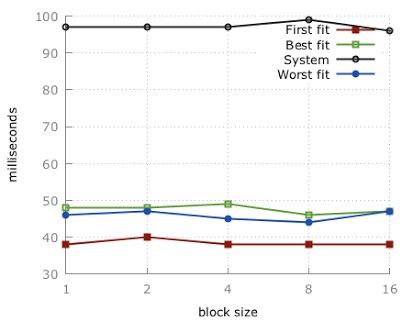
\includegraphics[width=1\textwidth]{images/time_plot_small1.png}
    \label{fig:p1}
    \captionof{figure}{\tiny{LOOPS = 20000, SIZE = 128}}
\end{minipage}%
\begin{minipage}{.5\textwidth}
    \centering
    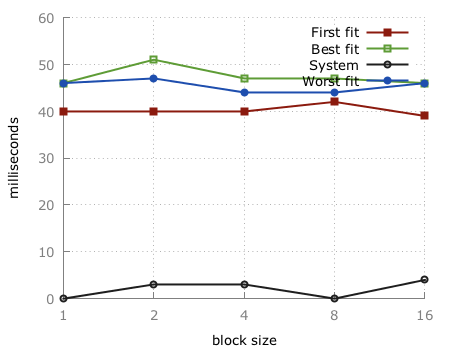
\includegraphics[width=1\textwidth]{images/time_plot_small2.png}
    \label{fig:p2}
    \captionof{figure}{\tiny{LOOPS = 20000, SIZE = 128}}
\end{minipage}\\\\

Ovanstående körningar hade samma parametrar. Våra algoritmer fick liknande resultat båda gångerna. First fit var något snabbare än best och worst fit. Systemets malloc hade ojämn prestanda vid små allokeringar. 
% kanske för diskussion..
Den dåliga körningstiden skulle bland annat kunna förklaras av att allokeringar av så små minnen är väldigt ovanligt. Systemets malloc innehåller dessutom en hel del funktionalitet som kräver initiering och hushållning.\\

För att vidare simulera vanlig användning körde vi ett test där vi allokerade slumpmässiga minnesstorlekar.
Storlekarna varierade från blockstorleken till blockstorleken*pagestorleken.
Man ser då en tydlig skillnad mellan de olika algoritmerna, där first-fit klarar sig bäst vid simulerad s.k. ``vanlig'' användning.

\begin{minipage}{.5\textwidth}
    \centering
    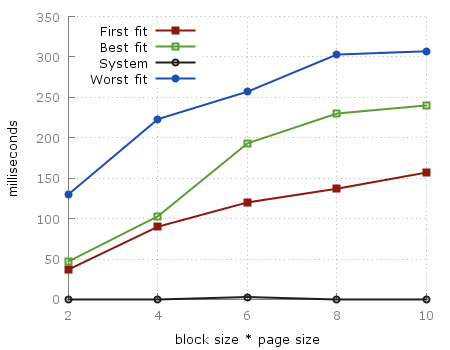
\includegraphics[width=1\textwidth]{images/time_plot_rand.png}
    \label{fig:p3}
    \captionof{figure}{\tiny{LOOPS = 20, SIZE = 128}}
\end{minipage}\\


\subsection{Stora allokeringar}


\subsection{Skydd av minne}

Vi implementerade skydd mot sönderskrivning av våra kontrollstrukturer. 
Detta åstadkom vi genom att ha en separat lista som håller reda på minne som |malloc| har allokerat.
Varje gång |free| anropas kontrolleras dess header genom att loopa över denna lista.
Om blocket inte finns i listan returneras |NULL|.

% bilder + förklaringar!

% Measurements from "Instruments" time profiler, Mac OS X.
% Fills an array of size 256, 10 000 times with the specified block size
% \begin{table}[h!] 
% \begin{tabular}{ c l l l}
%    Block size & First fit & Best fit & System malloc \\
%   \hline \\
%   1 & 57ms & 52ms & 24ms \\
%   2 & 49ms & 39ms & 29ms \\
%   4 & 51ms & 46ms & 30ms \\
%   8 & 58ms & 46ms & 25ms \\
%   16 & 39ms & 36ms & 33ms \\
% \end{tabular}
% \end{table}


%------------------------------------------------------------------------------
\section{Diskussion}

% synd att man inte kan mäta minne i system-malloc.

%------------------------------------------------------------------------------
\newpage
\section*{Appendix}
\subsection*{malloc.c}
\verbatiminput{../malloc.c}

\newpage
\subsection*{malloc.h}
\verbatiminput{../malloc.h}


\end{document}
